%%
%% Pilot report -- PPC 2026/27, English version.
%% Same format as the proposal (sample-sigchi.tex modified by DI/FCUL).
%% One page of text; page 2 holds Figure 1, Table 1 and the references.
%% Figure: python -m analysis.pilot_figures data/raw/campaign-v2 --output paper/figures
%%
\documentclass[sigplan]{acmart}
\settopmatter{printacmref=false}
\renewcommand\footnotetextcopyrightpermission[1]{}
\usepackage[english]{babel}
\usepackage{enumitem}

\begin{document}
\raggedbottom
\emergencystretch=1.5em

\title{Scalability of Parallel Code in WebAssembly in the Browser vs.\ Native: pilot report}

\author{David Coimbra - fc68024}
\affiliation{%
 \institution{
  Programação Paralela e Concorrente \\
  Mestrado em Engenharia Informática \\
  Faculdade de Ciências, Universidade de Lisboa}
 \country{Portugal}
 }
\email{fc68024@alunos.fc.ul.pt}

\begin{abstract}
The pilot built the harness and fixed the measurement configuration
from preliminary experiments. Without
synchronization WASM scales as natively; with shared atomics, scalability
depends on the engine.
\end{abstract}


\pagestyle{plain}

\maketitle

\noindent\textbf{Goals.}
\begin{description}[nosep]
  \item[RQ1] How do relative speedup and efficiency of the same Rust/Rayon
  code evolve with the number of threads, in WebAssembly in the browser and
  natively?
  \item[RQ2] To what extent does synchronization between threads affect
  the scalability gap observed in RQ1?
\end{description}
\noindent The study extends Kyriakou and Tselikas~\cite{kyriakou2022}, who
measured a single workload without synchronization.

\section{Environment and harness}

\noindent An i9-14900KF on Linux, turbo and SMT off, governor
\texttt{performance} (3.2~GHz). Chrome for
Testing 155 (V8; proposal: commercial Chrome; same engine, pinnable) and
Firefox 158 (SpiderMonkey).
One Rust/Rayon crate builds native and WASM with threads~\cite{haas2017},
128-bit SIMD on both; only the target features differ (WASM needs atomics,
always sequentially consistent~\cite{sanchez2025}). Workloads: a 3$\times$3 Gaussian
filter, and a histogram with shared atomics or with local counters (the
control). A CI/CD pipeline checks that the browser
checksums match the native ones.

\section{Measurement configuration}

\begin{itemize}[nosep,leftmargin=*]
  \item \textbf{Cores:} the 8 P-cores, one CPU mask for the whole process;
  no per-thread pinning, which a browser cannot do. P+E was slower and
  noisier.
  \item \textbf{Threads:} $N \in \{1,2,4,6,7,8\}$; 6 and 7 show whether the
  browser's own threads bend the curve near 8 cores.
  \item \textbf{Image $8192^2$}, 1~byte per pixel: iterations last at least
  100 times the browser clock resolution (5 to 20~\textmu s), and the
  64~MiB input and output exceed the 36~MiB L3 cache.
  \item \textbf{Warm-up $W$} per workload, equal in all environments: 1.5
  times the latest settling point in 100-iteration pilot runs (filter 15;
  atomic 5; local 15 to 71, the most at $k=1$).
  \item \textbf{30 runs} (fresh processes and browser profiles) of 10
  iterations per configuration and environment; a run is summarized by its
  median and is the unit of analysis~\cite{kalibera2013}. A 30-run pilot gave 99.5\% confidence intervals (CIs) within
  $\pm$1\% (RQ1) and $\pm$7.5\% (RQ2).
  \item \textbf{Browsers} headless, with a 3~s wait for Firefox's start-up.
  \item \textbf{Contention:} $k \in \{1,4,16,256\}$ distinct input values
  spread the increments over $k$ counters (proposal: noise vs.\ few
  colours). Atomic counters are padded to 128~bytes, one per cache line,
  also in WASM; the control counts per 64~KB task (proposal: per thread).
\end{itemize}

\section{Controls and analysis}

\begin{itemize}[nosep,leftmargin=*]
  \item Fixed-seed inputs; input fingerprint and output checksum per run;
  pinned browser versions~\cite{yan2021}; the system and harness off the
  measured cores.
  \item Pool created before the first iteration; every parallel region is
  started from outside the pool in both environments.
  Environments interleaved in a seeded random order~\cite{mytkowicz2009};
  runs with over 0.25~s of foreign CPU are excluded (threshold set from
  the pilots, before the campaign).
  \item Plan fixed before measuring: the run as the
  unit~\cite{georges2007}, bootstrap CIs~\cite{hoefler2015}, Holm
  correction over 10 primary contrasts at $N=8$. RQ1: the ratio of
  speedups. RQ2: $\exp(\Delta r)$, with $r=\log(T_\text{atomic}/
  T_\text{local})$ and $\Delta r$ the browser's $r$ minus the native one.
\end{itemize}

\section{Preliminary data}

\noindent Main campaign, 4860 runs (Fig.~\ref{fig:scaling},
Table~\ref{tab:rq2}). \textbf{RQ1.} The filter and the local histogram
scale close to ideal everywhere (Fig.~\ref{fig:scaling}a, c, e): filter
speedup at $N=8$ 7.04 native, 6.97 Chrome, 7.39 Firefox (efficiency 0.88,
0.87, 0.92); the ratio of speedups to native is 0.99 [0.95, 1.03] in
Chrome, no difference, and 1.05 [1.02, 1.07] in Firefox. Firefox's higher ratio comes from a slower $T_1$ (1.33 times native at
$N=1$, 1.27 at $N=8$; Fig.~\ref{fig:scaling}b), a WASM cost seen also
single-threaded~\cite{jangda2019}.

\textbf{RQ2.} Shared atomics at $k=1$ slow down with $N$ everywhere
(Fig.~\ref{fig:scaling}d). Synchronization costs Chrome up to 2.2 times
what it costs natively when contention is concentrated, and less than
natively at $k=256$ (0.42; Fig.~\ref{fig:scaling}f); Firefox is never
worse than native (0.79 to 0.99). In the machine code, V8 compiles the atomic
add to a \texttt{lock cmpxchg} retry loop; Firefox and native, to one
\texttt{lock add}~\cite{schweizer2015}; Chrome's advantage at $k=256$ is not
explained yet.

\begin{figure}[t]
\centering
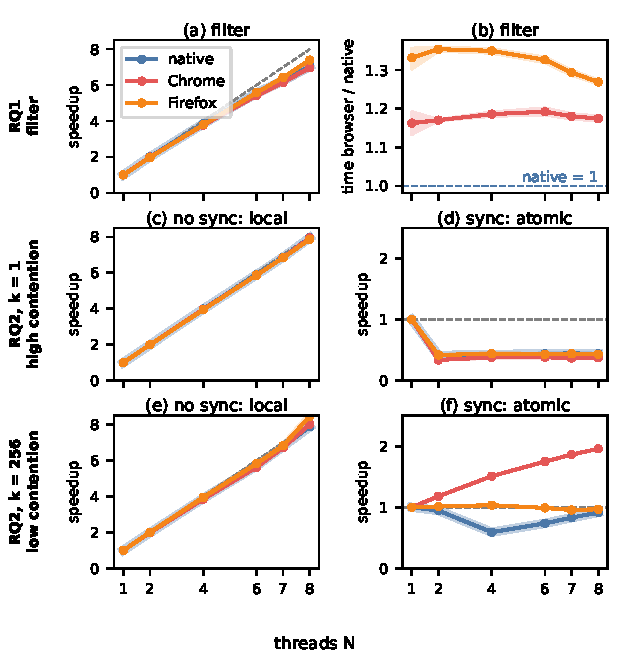
\includegraphics[width=\columnwidth]{../figures/pilot-scaling-en.pdf}
\caption{Main campaign, 30 runs per point, exploratory 95\% CI. Row 1:
RQ1, the filter's speedup $T_1/T_N$ and its time over native time. Rows 2
and 3: RQ2, speedup without (local) and with (atomic) synchronization, at
high ($k=1$) and low ($k=256$) contention. Dashed: ideal, or 1.}
\label{fig:scaling}
\end{figure}

\begin{table}[t]
\caption{RQ2 at $N=8$: $\exp(\Delta r)$ with the primary 99.5\% CI (above 1:
synchronization costs more than natively). *: rejected by Holm.}
\label{tab:rq2}
\small
\begin{tabular}{lcc}
\toprule
$k$ & Chrome & Firefox \\
\midrule
1   & 2.18 [2.04, 2.32]* & 0.99 [0.94, 1.05] \\
4   & 1.78 [1.75, 1.80]* & 0.97 [0.95, 0.98]* \\
16  & 1.45 [1.42, 1.47]* & 0.82 [0.80, 0.83]* \\
256 & 0.42 [0.41, 0.42]* & 0.79 [0.78, 0.81]* \\
\bottomrule
\end{tabular}
\end{table}

\noindent\textbf{Use of AI.} Claude helped with the design and reviewed the
text; the decisions are mine.

\bibliographystyle{ACM-Reference-Format}
\bibliography{../bib/referencias}

\end{document}
